\chapter{Travaux relatifs}
Autant la détection 3D est aboutie, autant la détection des éléments reste un sujet de recherche. Il existe donc deux approches différentes sur ce sujet : 

\section{Méthodes en 2D}
Projection de l’information en 2D se rapprochant de la méthode ARP, étudiée en ASI [Architecture des Systèmes d'Information] en quatrième année dans le cadre du cours de Data-Mining, pour réduire le temps de traitement. Cette méthode transforme une matrice de données de taille $\mathbb{R}^{N}$ en une matrice de données de taille $\mathbb{R}^{d}$ où $d<N$.


\section{Méthodes en 3D}

Le nuage de points 3D qui donne une vision panoramique. Proposé par Zhu et al. (2010) utilisant les données MLS [Multiple Listings Services]~\footnote{Partage de fichiers utilisés initialement pour le secteur immobilier et la communication entre vendeurs.} pour générer une \enquote{zone} panoramique dans laquelle chaque ligne représente le temps d’acquisition de chaque ligne laser, les colonnes représente l’ordre séquentiel de mesure et la valeur du pixel code la distance du capteur au point. Ils proposent une segmentation-classification à l’aide de graphes, SVM [Séparateurs à Vaste Marge]~\footnote{Les séparateurs à vaste marge sont un ensemble de techniques d'apprentissage supervisé destinées à résoudre des problèmes de discrimination et de régression}
et arbres de décision. Hernandez et Marcotegui (2009b) proposent une méthode projectant les données MLS en \enquote{image d'élévation}, c’est à dire, une vue de scène. Le sol, et les objets sont segmentés utilisant la transformation morphologique et classifiés en 4 catégories via la méthode SVM:
\begin{itemize}
\item Voitures
\item Lampes
\item Piétons
\item Autres
\end{itemize}

\begin{figure}[H]
\centering
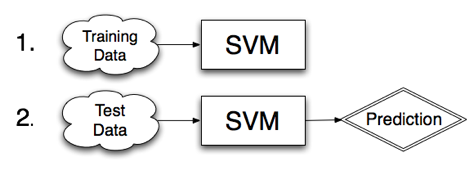
\includegraphics[width=0.5\linewidth]{./images/svm.png}
\caption{Schéma montrant l'utilisation de la méthode SVM dans le cadre de la prédiction via apprentissage supervisé}
\end{figure}